\documentclass{beamer}
\usetheme{Oxygen}
\usepackage{verbatim}
\usepackage{minted}

\title{Automated Code Transformation for Distributed Training of TensorFlow ML Models}
\author{Yusung Sim\inst{1}, Wonho Shin\inst{1}, Sungho Lee\inst{2}, Sukyoung Ryu\inst{1}}
\institute{
  \inst{1}%
  School of Computing, KAIST
  \and
  \inst{2}%
  Department of Computer Science and Engineering,\\ 
  Chungnam National University
}
\date{2022. 02. 10}

\begin{document}
% 0. Title
\frame{\titlepage}


% 1. Introduction
\begin{frame}{Reducing ML Training Time}
  \begin{definition}
    \textbf{Distributed training} is a machine learning(ML) technique
    that distributes the training computation 
    over \textit{multiple hardware devices}.
    (GPUs, TPUs, etc.)
  \end{definition}
  \begin{itemize}
    \item Distributed training reduces the training time.
    \item It is commonly used in academia and industry.
    \item Distributed training codes are often written in \textit{Horovod},\\
          a distributed training framework that supports \textit{TensorFlow}.  
  \end{itemize}
\end{frame}

\begin{frame}{Problem: Manual Rewriting}
  Single-GPU-based training codes should be converted into
  distributed training codes.
  \begin{itemize}
    \item Developers \textbf{manually rewrite} the training codes.
    \item This task is \textbf{labor-intensive} and \textbf{time-consuming}.
    \item It also requires an understanding of the model structure and Horovod framework.
  \end{itemize} 
\end{frame}

\begin{frame}{Solution: Automated Code Transformation for Distributed Training}
  We developed an \textbf{Automated Code Transformation SW}, which
  transforms a single-GPU-based training code into the distributed training code. 
  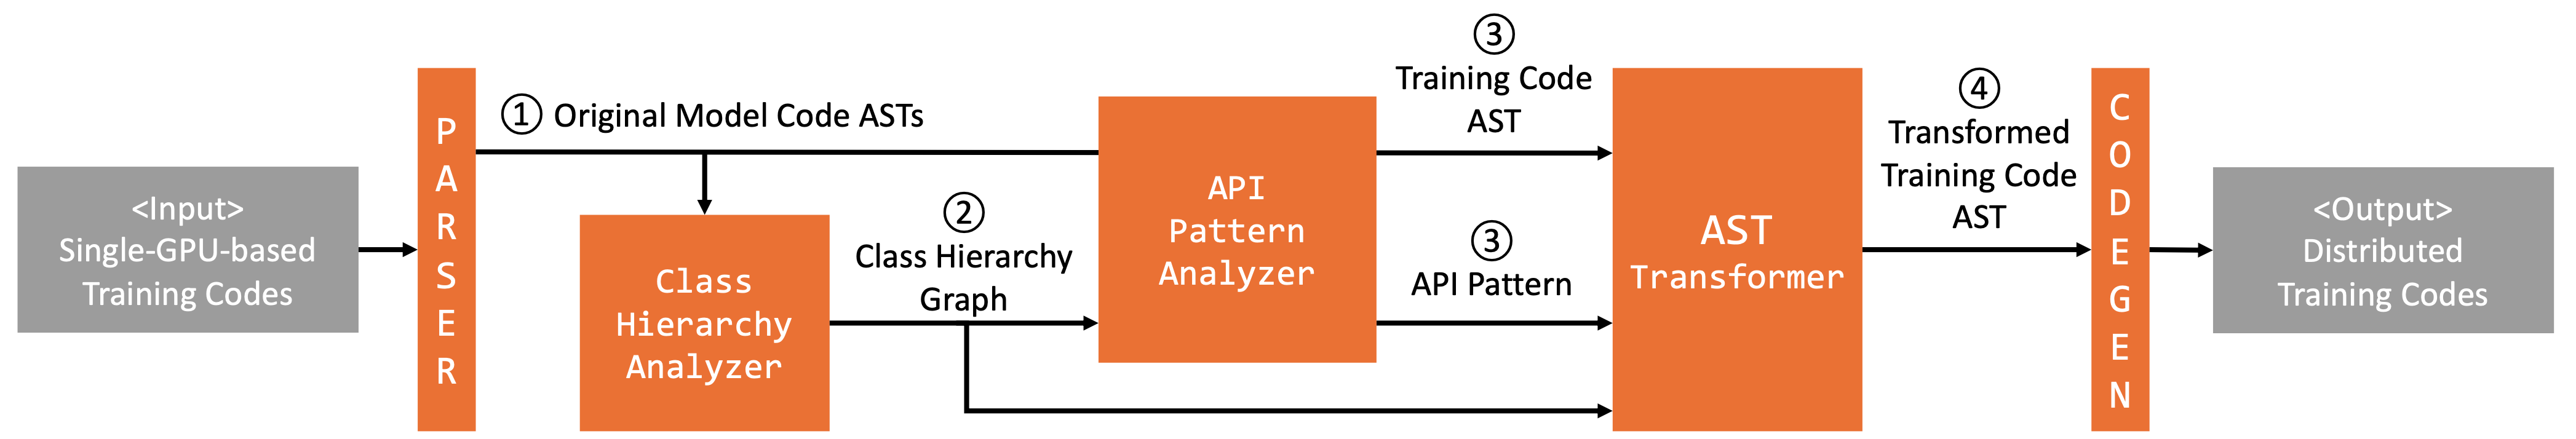
\includegraphics[width=\textwidth]{orange_arch} 

  {\scriptsize
  \begin{enumerate}
    \item Input model codes are parsed into ASTs. 
    \item Class hierarchy analyzer generates the model class hierarchy graph.
    \item API pattern analyzer finds the training code AST and its API pattern category.
    \item Given all the results, the AST transformer applies appropriate transformation
    on the training code AST.
    \item The transformed AST is printed out as a file. 
  \end{enumerate}
  }
\end{frame}

\begin{frame}{Challenges in Developing the Code Transformation SW}
  We faced two challenges in the development process.
  \begin{itemize}
    \item Identifying the \textbf{training API usage} to apply the correct transformation. 
    \item Recognizing \textbf{user-defined classes} that inherit TensorFlow classes.
  \end{itemize} 
\end{frame}

\begin{frame}{Challenge 1. Identifying Training Patterns}
  Tensorflow has multiple training APIs, and 
  different training APIs must be transformed in different ways.

  \begin{figure}
    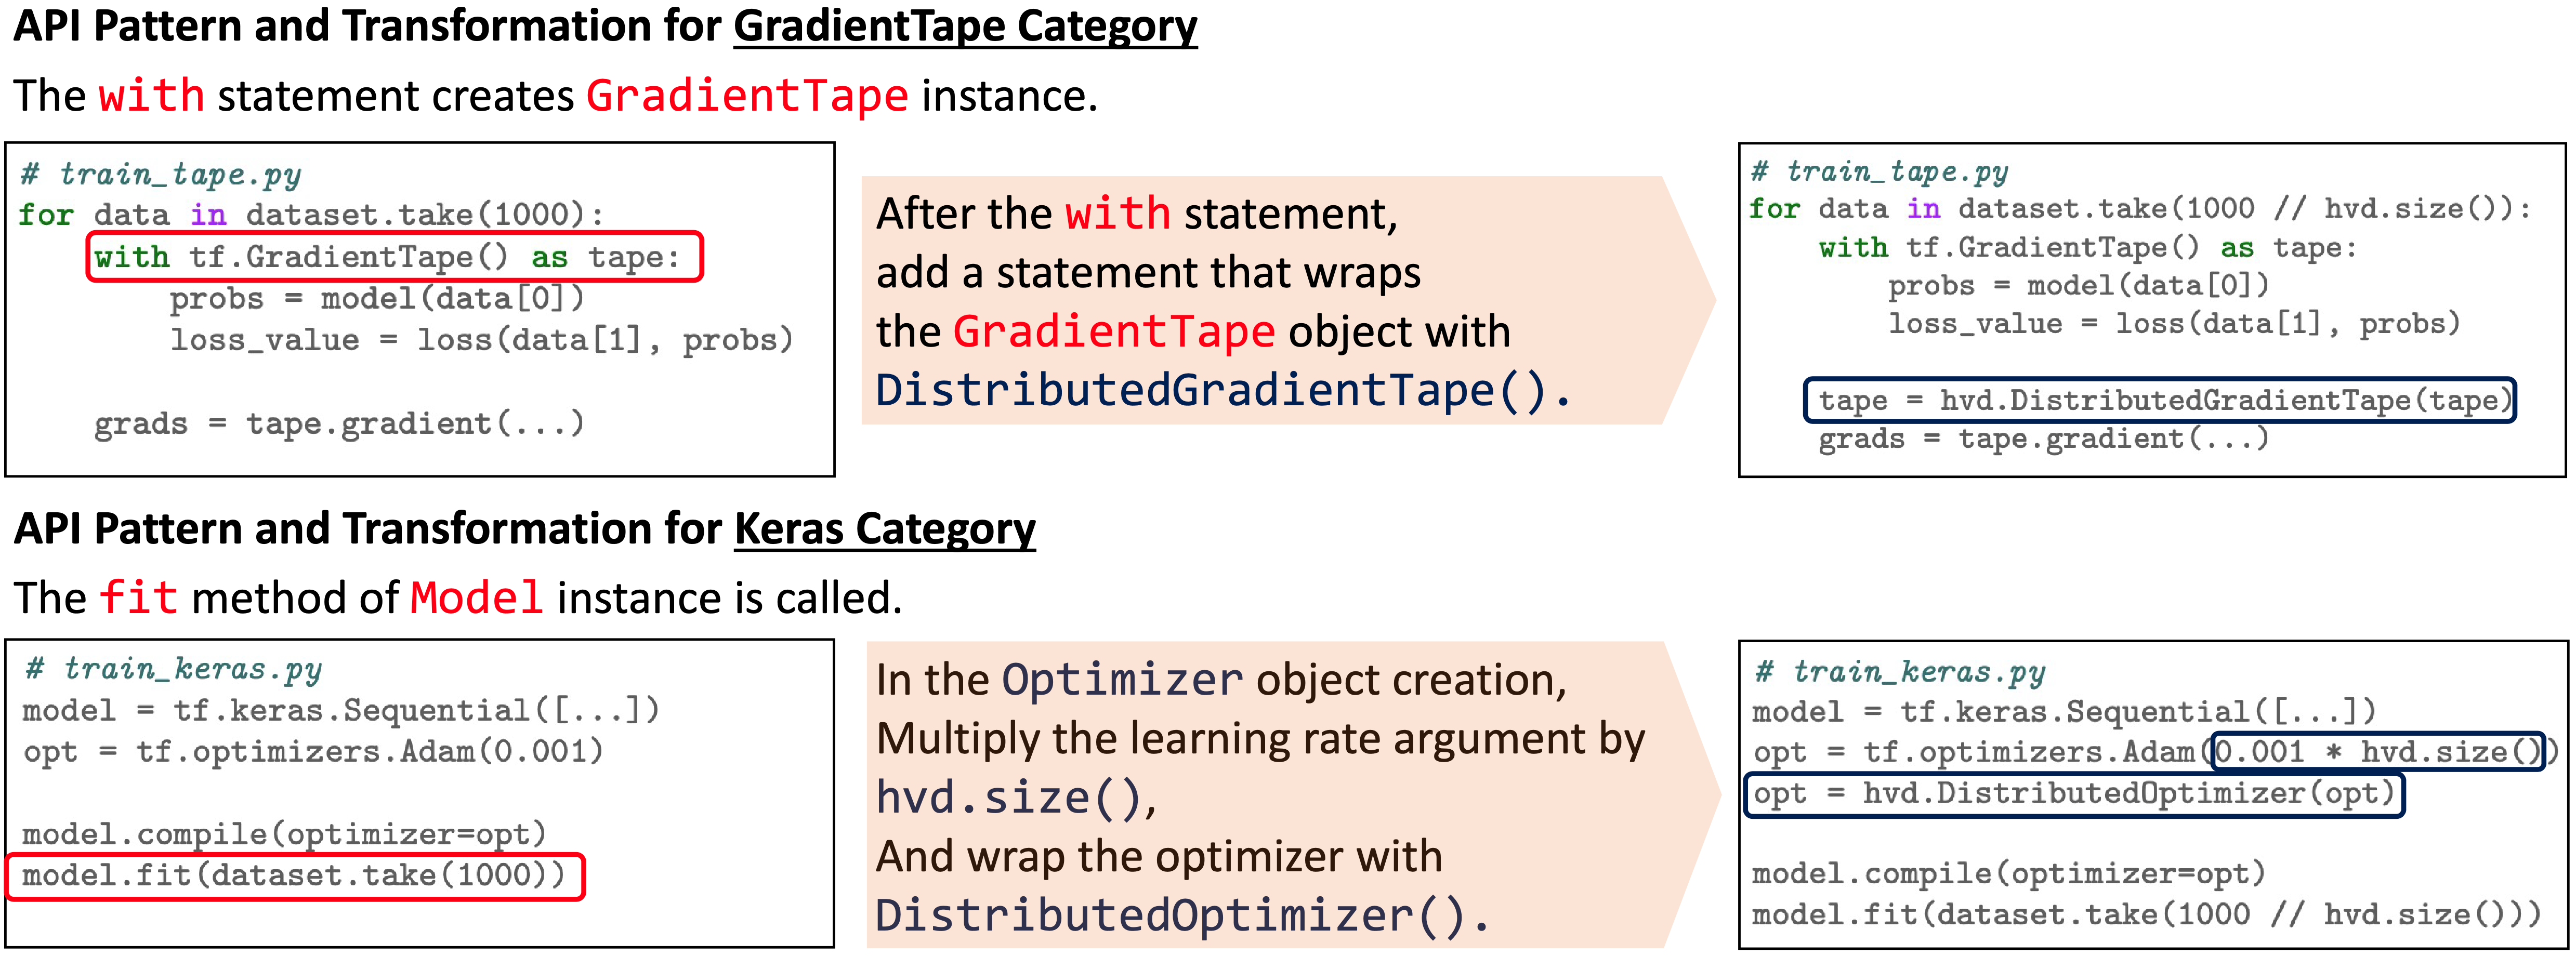
\includegraphics[width=\textwidth]{patternex} 
  \end{figure}
  {\footnotesize
    We match \textbf{training API patterns} to categorize the codes
    by their API usage and apply the correct transformation. 
  }
\end{frame}


\begin{frame}{Challenge 2. Recognizing User-defined Classes}
  User-defined classes inherit training-related classes in TensorFlow
  to extend their methods. (ex. {\tt Model.fit}) 

  \begin{figure}
    \centering
    
\includegraphics[width=0.6\textwidth]{revisedpattern}
    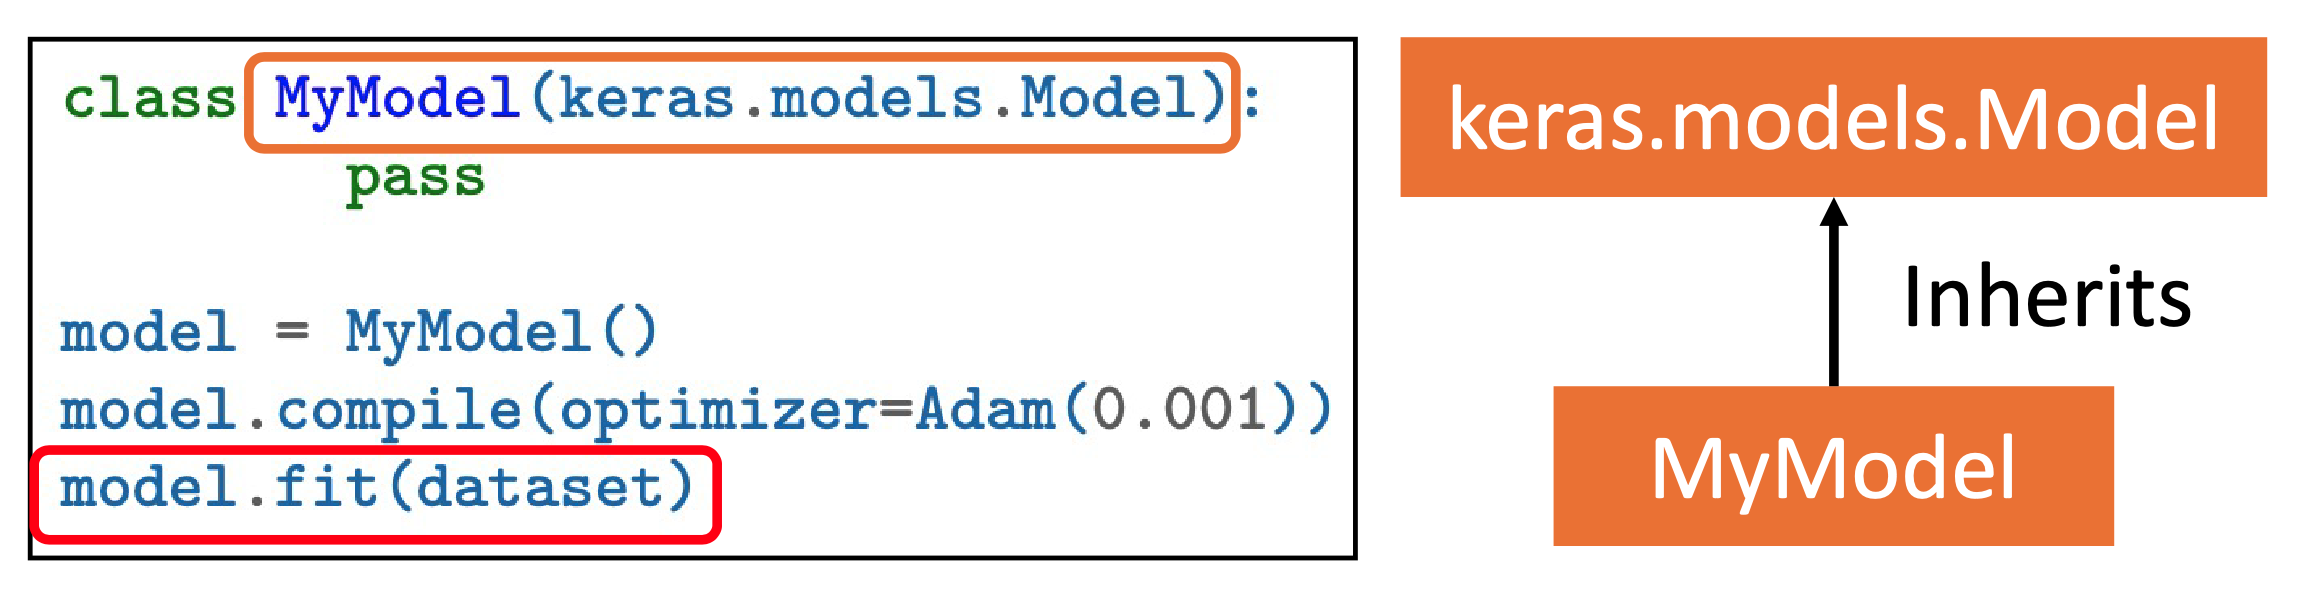
\includegraphics[width=0.7\textwidth]{chg}
  \end{figure}

  {\footnotesize
  \begin{itemize}
  \item API patterns and transformation rules are generalized
  in terms of the subclass relations. 
   
  \item The class hierarchy anlayzer
  constructs a \textbf{class hierarchy graph} to store the subclass relationships. 
  \end{itemize}
  }

\end{frame}

\begin{frame}{Results \& Future Works}
  \begin{figure}
    \begin{columns}
      \column{0.4\textwidth}
        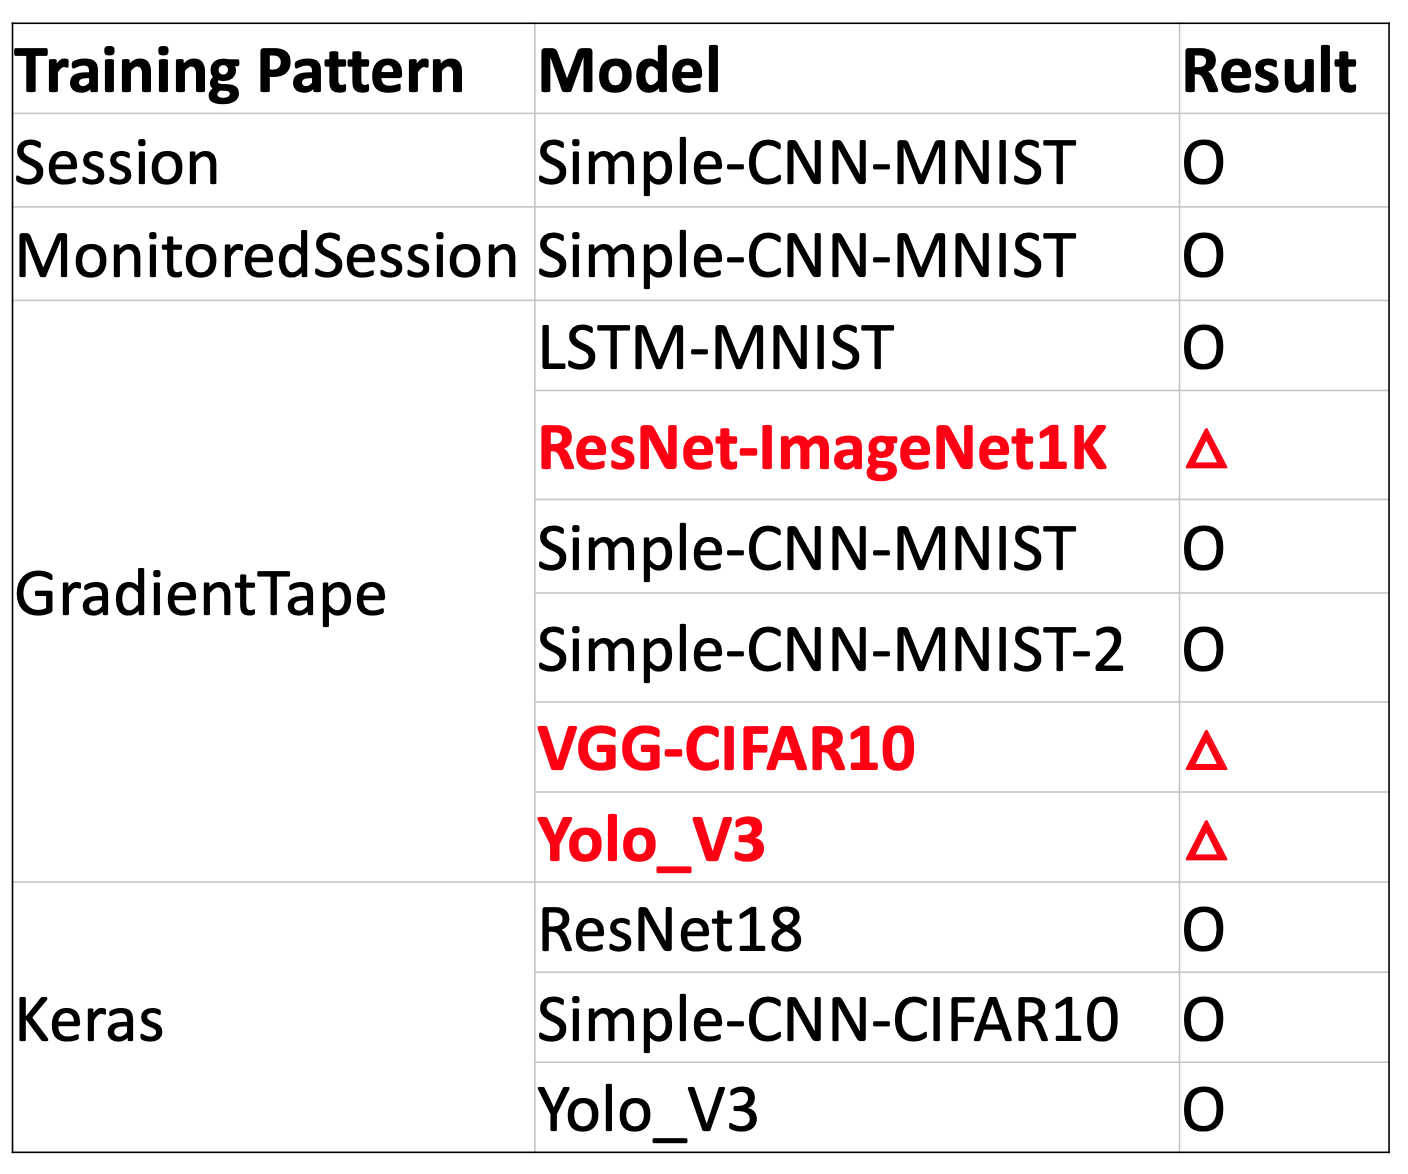
\includegraphics[width=1\textwidth]{results}
      \column{0.7\textwidth}
        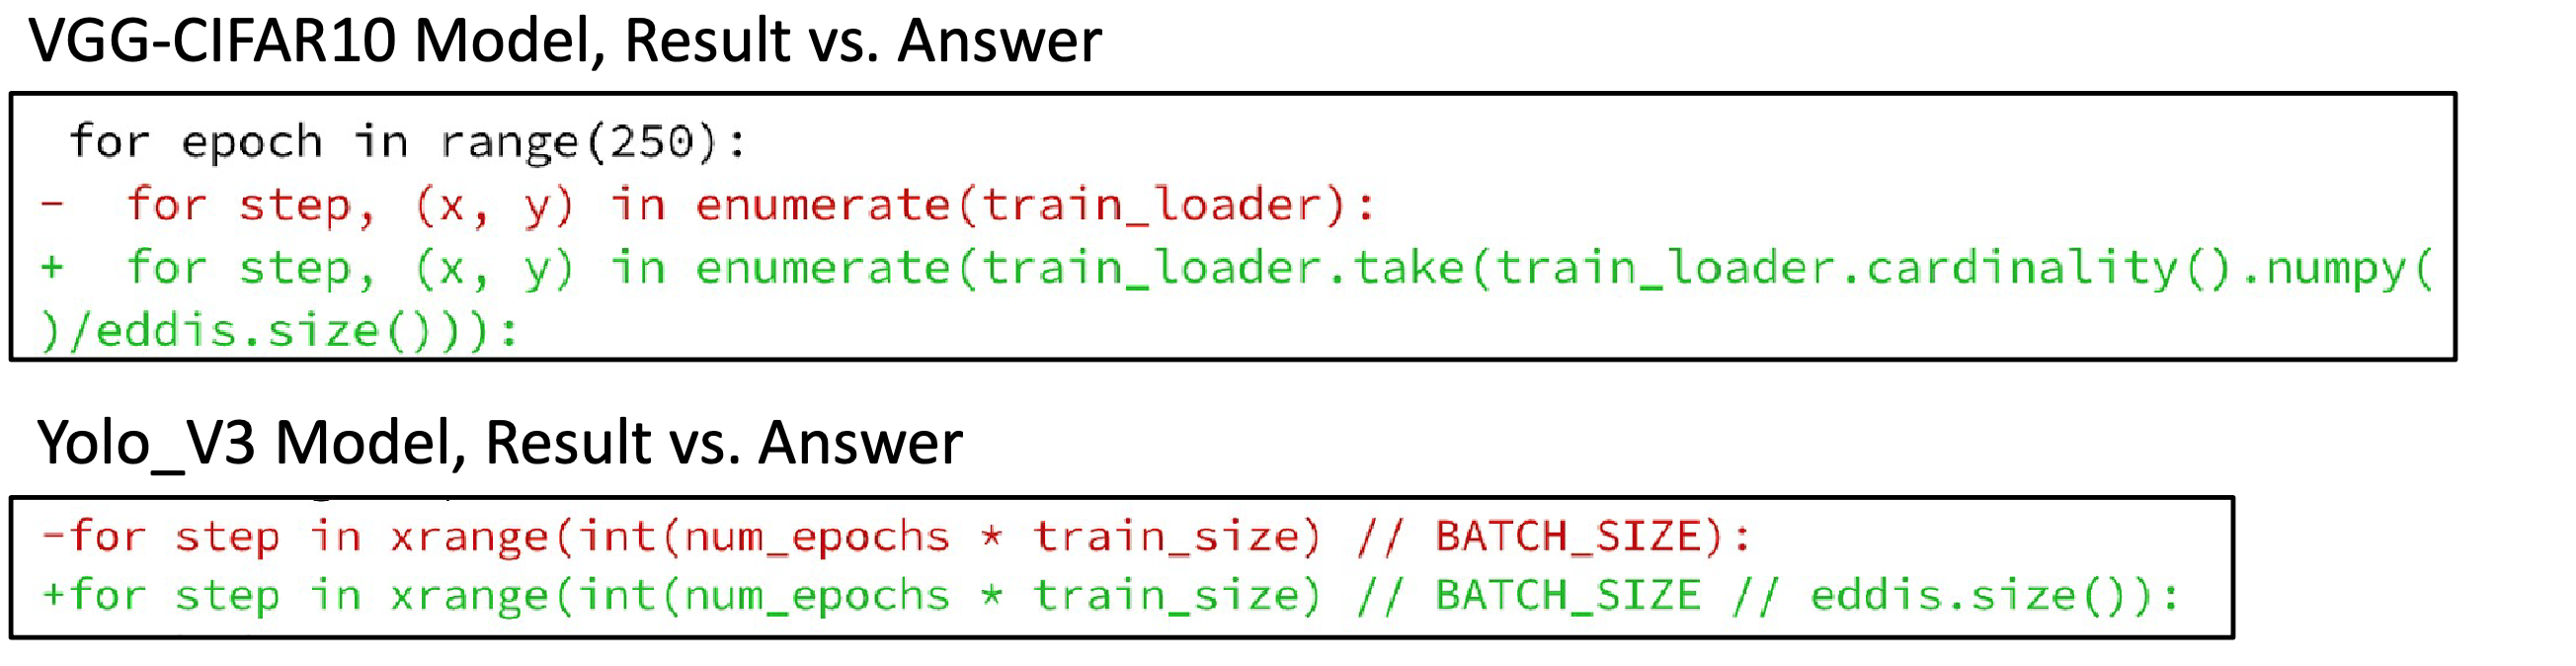
\includegraphics[width=1\textwidth]{trainstep}
    \end{columns}
  \end{figure}

  {\small
  \begin{itemize}
    \item We transformed \textbf{11 ML models} by the SW
          and compared them with manually crafted answers.\\
    \item 3 training codes are not fully transformed; 
          the numbers of training steps
          in the {\tt for} statements were not modified.
    \item In future work, we'll design a method to recognize
    \& modify the general form of the number of training steps. 
  \end{itemize}
  }

\end{frame}

\end{document}
